\documentclass{beamer}
\usepackage{graphicx}
\usepackage{hyperref}
\usepackage{diagbox}
\usepackage{colortbl}



\title{Online Outlier Exploration over Large Datasets}
\author{Matthias Hansen \\
        \texttt{matthias.hansen@rwth-aachen.de}}
\date{Data Mining and Multimedia Search}
\institute{RWTH Aachen University}
\begin{document}
\frame{\titlepage}

\begin{frame}{Motivation}
    \centering{Why do Outlier Detection?}
\end{frame}
\section{Outlier Detection}



\begin{frame}{Example: Gaussian Distribution $\mathcal{N}(0,1)$}
    \centering
    \includegraphics<1>[width=.7\textwidth]{images/gaussian.png}
    \includegraphics<2>[width=.7\textwidth]{images/gaussian_lines.png}

    \visible<2>{Within \alert{red} lines $\implies$ inlier.

    Outside \alert{red} lines $\implies$ outlier.}
\end{frame}

\begin{frame}{The Traditional Approach: Statistical Distributions}
    \begin{itemize}
        \item Statistical Distribution of Data must be known.
        \item Linear Runtime.
        \item Distribution can sometimes be Inferred (e.g. using Expectation Maximization).
    \end{itemize}
\end{frame}

\begin{frame}{Counterexample: Geospatial Data}
    \begin{itemize}
        \item OpenStreetMap Data for South America and South Pacific Islands

        \item Roughly 1.3 Gigabytes of Data. (Raw Positions)

        \item Obtained from \texttt{http://download.geofabrik.com}
    \end{itemize}
    \begin{center}
    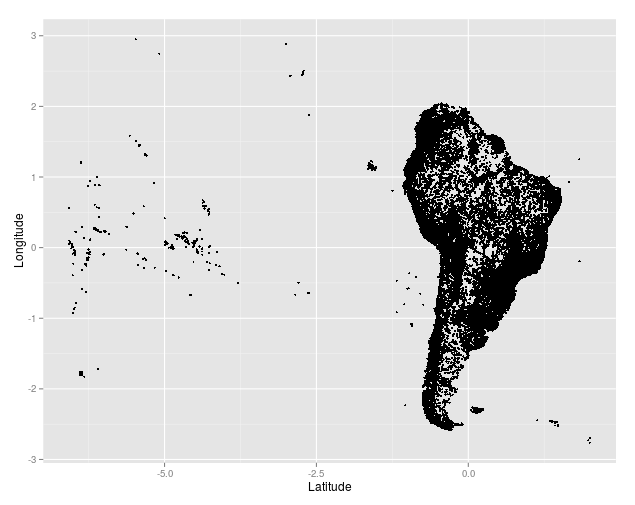
\includegraphics[width=.7\textwidth]{images/south_america.png} 
    \end{center}
\end{frame}

\begin{frame}
    \begin{center}
    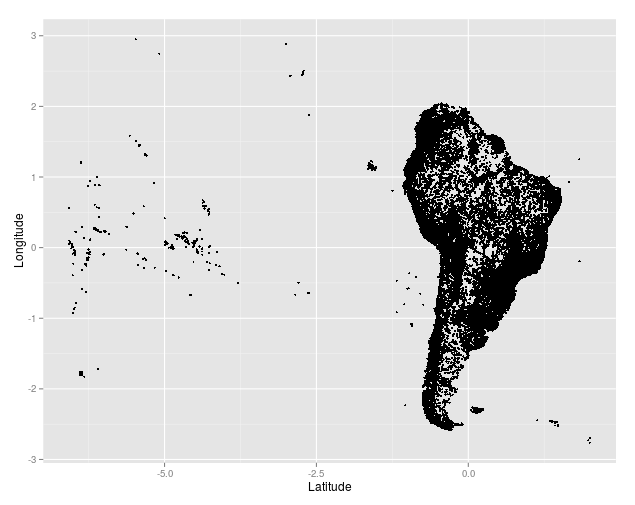
\includegraphics[width=.7\textwidth]{images/south_america.png} 
    \end{center}
    \begin{itemize}
        \item Task: Find wrong data inserted by malicious users.

        \item Example: Someone placed a shop in the middle of the ocean.

    \end{itemize}
\end{frame}

\begin{frame}{Distance-Based Outliers}
    \begin{block}{Distance-Based Outliers}
        Let DB be a sequence of vectors, dist a distance function.

        A point $p\in DB$ is a distance based outlier w.r.t. parameters $k$ and $\varepsilon$
        iff. $|\{q\in DB | dist(p,q) < \varepsilon\}| < k$
    \end{block}

    \begin{itemize}
        \item Same notion as ``non-core points'' in DBSCAN.
        \item Meaningful for geospatial data with Euclidean Distance.
    \end{itemize}
    %TODO add explanatory graphic here
\end{frame}

\section{Outlier Detection and Performance}
\begin{frame}{Performance Considerations}
    \begin{itemize}
        \item Naive way: Calculate pairwise distances. Then check criterion for each point.
        \item Better way: use a spatial Index structure to compute $k$-nearest neighbors. Check whether distance to $k$-th neighbor is $\leq$ $\varepsilon$.
        \item Runtime in $\mathcal{O}(n\log(n))$
    \end{itemize}
\end{frame}

\begin{frame}
    Select some parameters: \visible<2>{\alert{Maybe $k = 5$ and $\varepsilon = 0.0001$?}}
    \begin{center}
        \visible{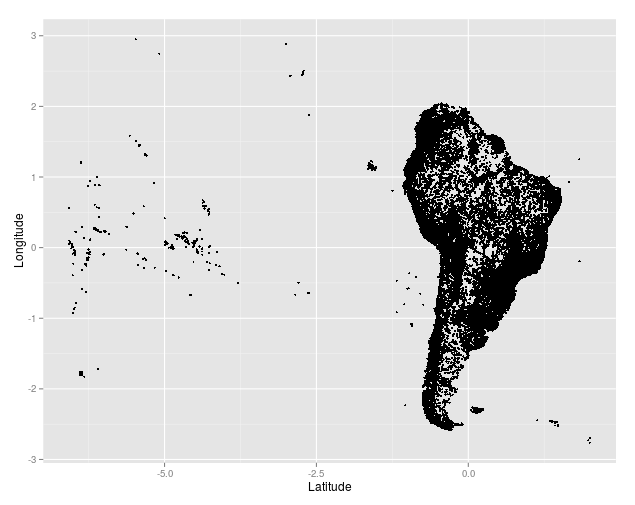
\includegraphics[width=\textwidth]{images/south_america.png}}
    \end{center}
\end{frame}

\begin{frame}
    Select some parameters: \alert{Maybe $k = 5$ and $\varepsilon = 0.0001$}?
    \begin{center}
        \visible{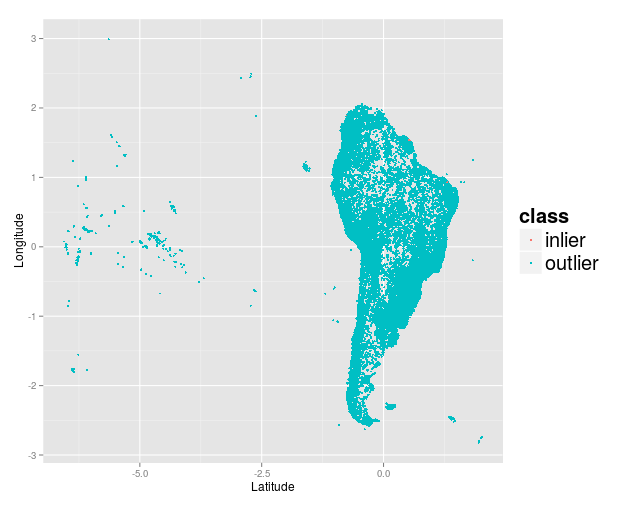
\includegraphics[width=\textwidth]{images/south_america_outliers.png}}
    \end{center}
\end{frame}

\begin{frame}{Parameter Selection is a Problem}
    \begin{itemize}
        \item Good parameter setting not obvious. 
        \item Settings can not be tested on Subsets: \alert{Results will differ!}
        \item Solution?
    \end{itemize}
\end{frame}


\begin{frame}{A Small Example}
    Consider the following dataset:
    \begin{columns}
        \begin{column}{.7\textwidth}
            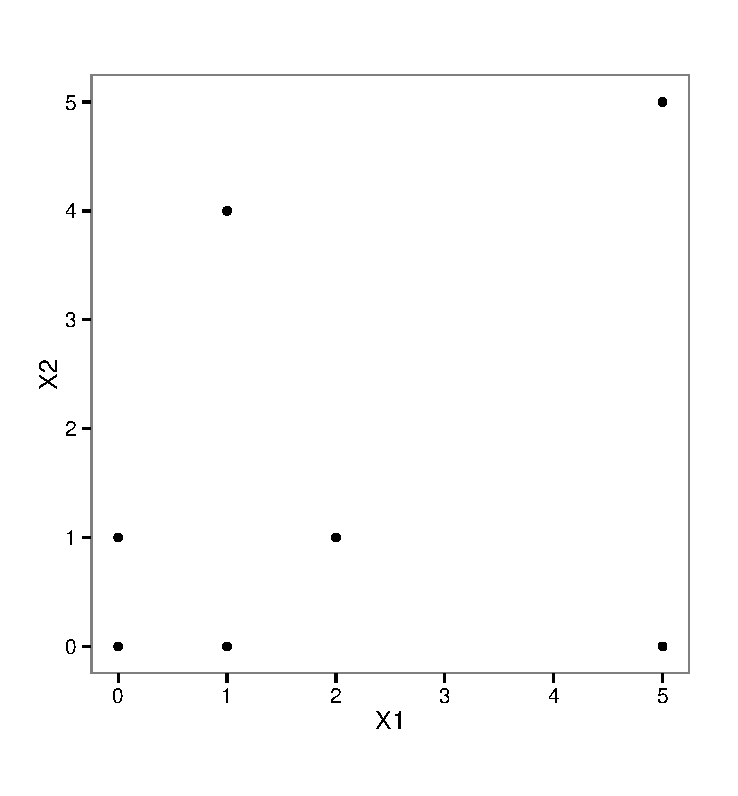
\includegraphics[width=.7\linewidth]{images/example_plot.eps}
        \end{column}
        \begin{column}{.3\textwidth}
            \begin{tabular}{ | c | c  c |}
            \hline
            i & X1 & X2 \\
            \hline
            0 & 0 & 0 \\
            1 & 1 & 0 \\
            2 & 0 & 1 \\
            3 & 5 & 0 \\
            4 & 1 & 4 \\
            5 & 2 & 1 \\
            6 & 5 & 5 \\
            \hline
            \end{tabular}
        \end{column}
    \end{columns}
    Say we want to perform outlier detection with $k=5$ and $\varepsilon=3.5$
\end{frame}
\begin{frame}
    Say we want to perform outlier detection with $k=5$ and $\varepsilon=3.5$
    $K$-Nearest-Neighbors query yields:
    \begin{tabular}{|c|c|c|c|c|c|}
        \hline
        \backslashbox{i}{k} & 1 & 2 & 3 & 4 & 5 \\
        \hline
        0 &  0 &  1.000000 &  1.000000 &  2.236068 &  4.123106\\
        1 &  0 &  1.000000 &  1.414214 &  1.414214 &  4.000000\\
        2 &  0 &  1.000000 &  1.414214 &  2.000000 &  3.162278\\
        3 &  0 &  3.162278 &  4.000000 &  5.000000 &  5.000000\\
        4 &  0 &  3.162278 &  3.162278 &  4.000000 &  4.123106\\
        5 &  0 &  1.414214 &  2.000000 &  2.236068 &  3.162278\\
        6 &  0 &  4.123106 &  5.000000 &  5.000000 &  6.403124\\
        \hline
     \end{tabular}
\end{frame}
\begin{frame}
    Say we want to perform outlier detection with $k=5$ and $\varepsilon=3.5$
    $K$-Nearest-Neighbors query yields:
    \begin{tabular}{|c|c|c|c|c|>{\columncolor[rgb]{1,0.5,0.5}}c|}
        \hline
        \backslashbox{i}{k} & 1 & 2 & 3 & 4 & 5 \\
        \hline
        0 &  0 &  1.000000 &  1.000000 &  2.236068 &  4.123106\\
        1 &  0 &  1.000000 &  1.414214 &  1.414214 &  4.000000\\
        2 &  0 &  1.000000 &  1.414214 &  2.000000 &  3.162278\\
        3 &  0 &  3.162278 &  4.000000 &  5.000000 &  5.000000\\
        4 &  0 &  3.162278 &  3.162278 &  4.000000 &  4.123106\\
        5 &  0 &  1.414214 &  2.000000 &  2.236068 &  3.162278\\
        6 &  0 &  4.123106 &  5.000000 &  5.000000 &  6.403124\\
        \hline
     \end{tabular}
\end{frame}
\end{document}
